\subsection{Gestione magazzini: Jolie}
L'implementazione della gestione dei magazzini \`e stata fatta
utilizzando una SOA di servizi Jolie. I file utilizzati sono quelli
contenuti nella directory \linebreak {\tt Magazzino}.
La gestione del magazzino viene dunque implementata utilizzando tre
componenti principali: 
\begin{itemize}
  \item magazzino primario, suddiviso in:
    \begin{itemize}
      \item interfaccia ({\tt interfMagazzinoPrimario.iol});
      \item implementazione ({\tt magazzinoPrimario.ol});
    \end{itemize}
  \item magazzini secondari, suddivisi in:
    \begin{itemize}
      \item interfaccia ({\tt interfMagazzinoSecondario.iol});
      \item implementazione ({\tt magazzinoSecondarioX.iol});
    \end{itemize}
  \item tipi di dato utili alle operazioni ({\tt dataTypes.iol}).
\end{itemize}

\subsubsection*{\tt intefMagazzinoPrimario.iol}
Interfaccia che contiene le operazioni che possono essere effettuate dal
magazzino primario. Le operazioni sono tutte del tipo
{\tt RequestResponse}, come mostrato in figura. \\\\
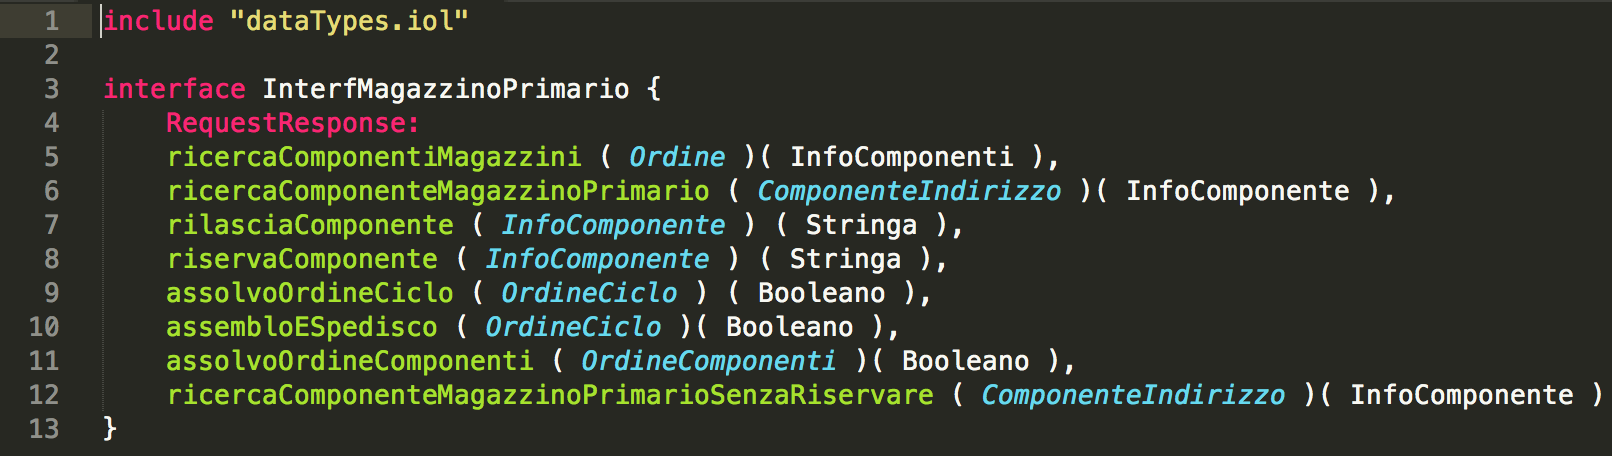
\includegraphics[scale=0.4]{immagini/interfMagazzinoPrimario.png}

\subsubsection*{\tt magazzinoPrimario.ol}
Questo file contiene l'implementazione delle operazioni del magazzino
primario. Contiene una {\tt inputPort}, in ascolto sulla porta {\tt 8000}
utilizzando un protocollo {\tt soap}, ed una serie di {\tt outputPort},
per gestire le interazioni con:
\begin{itemize}
  \item se stesso ({\tt soap}, {\tt 8000});
  \item il primo magazzino secondario ({\tt soap}, {\tt 8001});
  \item il secondo magazzino secondario ({\tt soap}, {\tt 8002});
  \item il servizio di calcolo delle distanze ({\tt http}, {\tt 8100});
  \item il servizio del fornitore ({\tt http}, {\tt 8300});
  \item il servizio di corriere ({\tt http}, {\tt 8400}).
\end{itemize}
Viene poi creata una procedura di {\tt init}, nel quale vengono
inizializzate le informazioni principali: le informazioni del magazzino
primario, le informazioni dei magazzini secondari e il listino delle
componenti presenti nel magazzino secondario.

I magazzini implementano un sistema elementare per simulare la presenza
dei componenti al loro interno, in modo da permettere di effettuare test
dei meccanismi di ricerca, di riserva componenti e di calcolo delle
distanze. Non viene utilizzato un database, poich\'e non necessario per
mostrare le caratteristiche del sistema.

Vengono poi implementate le operazioni definite nell'interfaccia;
alcune di queste operazioni eseguono solamente compiti fittizi,
semplificazioni dei meccanismi del mondo reale:
\begin{itemize}
  \item {\tt rilasciaComponente}: si limita semplicemente a stampare una
  componente riservata, indicando per esempio in che magazzino si trova,
  delegando a questo il rilascio effettivo (che consiste nella stampa di
  una stringa);
  \item {\tt riservaComponenti}: ha un funzionamento analogo a quello
  della funzione precedente;
  \item {\tt assembloESpedisco}: per simulare le attivit\`a effettive di
  un'officina viene generata una richiesta di spedizione con i dati del
  prodotto (un identificativo intero generato casualmente tramite
  l'interfaccia {\tt Math} offerta da Jolie) e i dati del cliente.
  Vengono stampate stringhe per simulare l'assemblaggio del cliclo; si
  attende poi la risposta della ditta di spedizioni per quanto riguarda
  l'esito della spedizione al cliente.
\end{itemize}
Altre operazioni hanno invece un'implementazione pi\`u realistica,
poich\'e rappresentavano problemi centrali per la soluzione. Queste
sono:
\begin{itemize}
  \item {\tt ricercaComponentiMagazzini}: questa operazione, presa una
  lista di componenti, le ricerca all'interno di tutti i magazzini.
  Restituisce una lista di componenti con la loro ubicazione (scelta
  prendendo la pi\`u vicina al cliente). I componenti trovati vengono
  riservati. Interagisce sia con il magazzino primario che con quelli
  secondari;
  \item {\tt ricercaComponenteMagazzinoPrimario}: presa una componente,
  restituisce le informazioni ricavate dalla ricerca all'interno del
  magazzino primario. Utilizza il servizio di calcolo delle distanze e,
  in caso di successo nella ricerca, l'operazione
  {\tt riservaComponenti};
  \item {\tt assolvoOrdineCiclo}: preso un elenco di componenti, vengono
  ricercate all'interno del magazzino primario (senza riservarle); se la
  componente non viene trovata, viene cercata nei magazzini secondari.
  Se l'esito di questa ricerca \`e positivo, si simuler\`a la spedizione
  al magazzino primario tramite l'operazione
  {\tt spedisciAlMagazzinoPrimario}. Altrimenti la componente viene
  ordinata al fornitore tramite l'operazione {\tt richiestaOrdine}. Si
  occupa inoltre di assemblare il ciclo e di spedirlo;
  \item {\tt assolvoOrdineComponenti}: preso un elenco di componenti,
  verifica il campo booleano che determina la necessit\`a di ordinare
  componenti. Nel caso ci sia, si chiama l'operazione
  {\tt richiestaOrdine} del fornitore. Finito il controllo e gli
  eventuali ordini, si chiama l'operazione \linebreak
  {\tt richiestaSpedizione}, dando al corriere come indirizzo di
  partenza quello del magazzino indicato nelle informazioni della
  singola componente.
\end{itemize}

\subsubsection*{\tt intefMagazzinoSecondario.iol}
Interfaccia che contiene tutte le operazioni che possono essere
effettuate dai magazzini secondari. Questa interfaccia \`e comune a
tutti i magazzini secondari. Le operazioni sono tutte del tipo
{\tt RequestResponse}, come mostrato in figura. \\\\
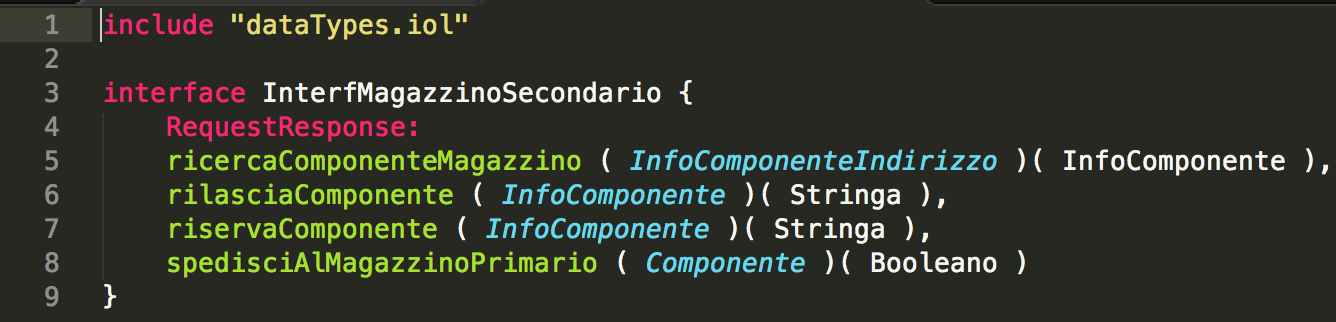
\includegraphics[scale=0.5]{immagini/interfMagazzinoSecondario.png}

\subsubsection*{\tt magazzinoSecondario[x].ol}
Mentre il file di interfaccia dei magazzini secondari \`e unico per
tutti, le implementazioni sono tante quanti sono i magazzini secondari.

Come si pu\`o intuire, utilizzando questo meccanismo, aggiungere o
cancellare un magazzino secondario diventa un'operazione estremamente
semplice: basta aggiungere/eliminare il file
{\tt magazzinoSecondario[x].ol} corrispondente ed aggiungere/eliminare
le informazioni e l'{\tt OutputPort} all'interno del file di
implementazione del magazzino primario.
Contiene una {\tt inputPort}, in ascolto sulla porta {\tt 800[x]} con
protocollo {\tt soap}, ed una serie di {\tt outputPort}, per gestire le
interazioni con:
\begin{itemize}
  \item il magazzino primario ({\tt soap}, {\tt 8000});
  \item il servizio di calcolo delle distanze ({\tt http}, {\tt 8100}).
\end{itemize}
Non sono contemplate interazioni con altri magazzini secondari, poich\'e
la coordinazione viene completamente gestita dal magazzino primario.

Viene poi creata una procedura di {\tt init}, nella quale si definiscono
le informazioni del magazzino, come id, indirizzo e listino delle
componenti presenti.
Vengono poi implementate le operazioni definite nell'interfaccia:
\begin{itemize}
  \item {\tt ricercaComponenteMagazzino}: \linebreak
  analoga all'operazione {\tt ricercaComponenteMagazzinoPrimario},\\ con
  l'unica differenza che, in caso che la componente sia presente e il
  \linebreak
  magazzino sia pi\`u vicino al cliente di quanto lo fosse il magazzino
  precedente (indicato nelle informazioni della componente), viene
  chiamata \linebreak l'operazione {\tt rilasciaComponente} sul
  magazzino precedente;
  \item {\tt rilasciaComponente}: si limita a restituire una stringa con
  notifica di successo;
  \item {\tt riservaComponente}: analoga alla {\tt rilasciaComponente};
  \item {\tt spedisciAlMagazzinoPrimario}: simula la spedizione dei
  componenti al magazzino primario.
\end{itemize}

\subsubsection*{\tt dataTypes.iol}
Questo file contiene i tipi di dato che verranno utilizzati all'interno
della soluzione.
Gli ultimi due tipi, {\tt Booleano} e {\tt Stringa} sono stati creati
per la generazione dei file \textit{wsdl}, che non consentono tipi
semplici nei parametri in ingresso ed uscita delle operazioni.

